\documentclass[]{article}
\usepackage{lmodern}
\usepackage{amssymb,amsmath}
\usepackage{ifxetex,ifluatex}
\usepackage{fixltx2e} % provides \textsubscript
\ifnum 0\ifxetex 1\fi\ifluatex 1\fi=0 % if pdftex
  \usepackage[T1]{fontenc}
  \usepackage[utf8]{inputenc}
\else % if luatex or xelatex
  \ifxetex
    \usepackage{mathspec}
  \else
    \usepackage{fontspec}
  \fi
  \defaultfontfeatures{Ligatures=TeX,Scale=MatchLowercase}
\fi
% use upquote if available, for straight quotes in verbatim environments
\IfFileExists{upquote.sty}{\usepackage{upquote}}{}
% use microtype if available
\IfFileExists{microtype.sty}{%
\usepackage{microtype}
\UseMicrotypeSet[protrusion]{basicmath} % disable protrusion for tt fonts
}{}
\usepackage[margin=1in]{geometry}
\usepackage{hyperref}
\hypersetup{unicode=true,
            pdftitle={MSc. Research Methods - Statistikteil Lösungen 2018},
            pdfauthor={Gian-Andrea Egeler},
            pdfborder={0 0 0},
            breaklinks=true}
\urlstyle{same}  % don't use monospace font for urls
\usepackage{color}
\usepackage{fancyvrb}
\newcommand{\VerbBar}{|}
\newcommand{\VERB}{\Verb[commandchars=\\\{\}]}
\DefineVerbatimEnvironment{Highlighting}{Verbatim}{commandchars=\\\{\}}
% Add ',fontsize=\small' for more characters per line
\usepackage{framed}
\definecolor{shadecolor}{RGB}{248,248,248}
\newenvironment{Shaded}{\begin{snugshade}}{\end{snugshade}}
\newcommand{\AlertTok}[1]{\textcolor[rgb]{0.94,0.16,0.16}{#1}}
\newcommand{\AnnotationTok}[1]{\textcolor[rgb]{0.56,0.35,0.01}{\textbf{\textit{#1}}}}
\newcommand{\AttributeTok}[1]{\textcolor[rgb]{0.77,0.63,0.00}{#1}}
\newcommand{\BaseNTok}[1]{\textcolor[rgb]{0.00,0.00,0.81}{#1}}
\newcommand{\BuiltInTok}[1]{#1}
\newcommand{\CharTok}[1]{\textcolor[rgb]{0.31,0.60,0.02}{#1}}
\newcommand{\CommentTok}[1]{\textcolor[rgb]{0.56,0.35,0.01}{\textit{#1}}}
\newcommand{\CommentVarTok}[1]{\textcolor[rgb]{0.56,0.35,0.01}{\textbf{\textit{#1}}}}
\newcommand{\ConstantTok}[1]{\textcolor[rgb]{0.00,0.00,0.00}{#1}}
\newcommand{\ControlFlowTok}[1]{\textcolor[rgb]{0.13,0.29,0.53}{\textbf{#1}}}
\newcommand{\DataTypeTok}[1]{\textcolor[rgb]{0.13,0.29,0.53}{#1}}
\newcommand{\DecValTok}[1]{\textcolor[rgb]{0.00,0.00,0.81}{#1}}
\newcommand{\DocumentationTok}[1]{\textcolor[rgb]{0.56,0.35,0.01}{\textbf{\textit{#1}}}}
\newcommand{\ErrorTok}[1]{\textcolor[rgb]{0.64,0.00,0.00}{\textbf{#1}}}
\newcommand{\ExtensionTok}[1]{#1}
\newcommand{\FloatTok}[1]{\textcolor[rgb]{0.00,0.00,0.81}{#1}}
\newcommand{\FunctionTok}[1]{\textcolor[rgb]{0.00,0.00,0.00}{#1}}
\newcommand{\ImportTok}[1]{#1}
\newcommand{\InformationTok}[1]{\textcolor[rgb]{0.56,0.35,0.01}{\textbf{\textit{#1}}}}
\newcommand{\KeywordTok}[1]{\textcolor[rgb]{0.13,0.29,0.53}{\textbf{#1}}}
\newcommand{\NormalTok}[1]{#1}
\newcommand{\OperatorTok}[1]{\textcolor[rgb]{0.81,0.36,0.00}{\textbf{#1}}}
\newcommand{\OtherTok}[1]{\textcolor[rgb]{0.56,0.35,0.01}{#1}}
\newcommand{\PreprocessorTok}[1]{\textcolor[rgb]{0.56,0.35,0.01}{\textit{#1}}}
\newcommand{\RegionMarkerTok}[1]{#1}
\newcommand{\SpecialCharTok}[1]{\textcolor[rgb]{0.00,0.00,0.00}{#1}}
\newcommand{\SpecialStringTok}[1]{\textcolor[rgb]{0.31,0.60,0.02}{#1}}
\newcommand{\StringTok}[1]{\textcolor[rgb]{0.31,0.60,0.02}{#1}}
\newcommand{\VariableTok}[1]{\textcolor[rgb]{0.00,0.00,0.00}{#1}}
\newcommand{\VerbatimStringTok}[1]{\textcolor[rgb]{0.31,0.60,0.02}{#1}}
\newcommand{\WarningTok}[1]{\textcolor[rgb]{0.56,0.35,0.01}{\textbf{\textit{#1}}}}
\usepackage{longtable,booktabs}
\usepackage{graphicx,grffile}
\makeatletter
\def\maxwidth{\ifdim\Gin@nat@width>\linewidth\linewidth\else\Gin@nat@width\fi}
\def\maxheight{\ifdim\Gin@nat@height>\textheight\textheight\else\Gin@nat@height\fi}
\makeatother
% Scale images if necessary, so that they will not overflow the page
% margins by default, and it is still possible to overwrite the defaults
% using explicit options in \includegraphics[width, height, ...]{}
\setkeys{Gin}{width=\maxwidth,height=\maxheight,keepaspectratio}
\IfFileExists{parskip.sty}{%
\usepackage{parskip}
}{% else
\setlength{\parindent}{0pt}
\setlength{\parskip}{6pt plus 2pt minus 1pt}
}
\setlength{\emergencystretch}{3em}  % prevent overfull lines
\providecommand{\tightlist}{%
  \setlength{\itemsep}{0pt}\setlength{\parskip}{0pt}}
\setcounter{secnumdepth}{0}
% Redefines (sub)paragraphs to behave more like sections
\ifx\paragraph\undefined\else
\let\oldparagraph\paragraph
\renewcommand{\paragraph}[1]{\oldparagraph{#1}\mbox{}}
\fi
\ifx\subparagraph\undefined\else
\let\oldsubparagraph\subparagraph
\renewcommand{\subparagraph}[1]{\oldsubparagraph{#1}\mbox{}}
\fi

%%% Use protect on footnotes to avoid problems with footnotes in titles
\let\rmarkdownfootnote\footnote%
\def\footnote{\protect\rmarkdownfootnote}

%%% Change title format to be more compact
\usepackage{titling}

% Create subtitle command for use in maketitle
\newcommand{\subtitle}[1]{
  \posttitle{
    \begin{center}\large#1\end{center}
    }
}

\setlength{\droptitle}{-2em}

  \title{MSc. Research Methods - Statistikteil Lösungen 2018}
    \pretitle{\vspace{\droptitle}\centering\huge}
  \posttitle{\par}
    \author{Gian-Andrea Egeler}
    \preauthor{\centering\large\emph}
  \postauthor{\par}
      \predate{\centering\large\emph}
  \postdate{\par}
    \date{October 2019}


\begin{document}
\maketitle

\hypertarget{ubung-1.2-chi2-test}{%
\subsubsection{\texorpdfstring{Übung 1.2:
\(\chi^2\)-Test}{Übung 1.2: \textbackslash{}chi\^{}2-Test}}\label{ubung-1.2-chi2-test}}

\(H_0\): Es gibt keine Unterschiede zwischen der Population und der
Stichprobe bezüglich Geschlecht und Hochschulzugehörigkeit.

\par

\(H_1\): Es gibt Unterschiede zwischen der Population und der Stichprobe
bezüglich Geschlecht und Hochschulzugehörigkeit.

\begin{Shaded}
\begin{Highlighting}[]
\CommentTok{# gruppiert die Varieblen und fasst sie }
\CommentTok{# nach Geschlecht und Hochschulzugehörigkeit zusammen }

\NormalTok{canteen <-}\StringTok{ }\KeywordTok{group_by}\NormalTok{(nova, gender, member) }\OperatorTok\StringTok{ }
\StringTok{  }\KeywordTok{summarise}\NormalTok{(}\DataTypeTok{tot =} \KeywordTok{n}\NormalTok{()) }\OperatorTok\StringTok{ }
\StringTok{  }\KeywordTok{ungroup}\NormalTok{() }\OperatorTok
\StringTok{  }\KeywordTok{mutate}\NormalTok{(}\DataTypeTok{canteen_member =} \KeywordTok{c}\NormalTok{(}\StringTok{"Mitarbeiterinnen"}\NormalTok{, }\StringTok{"Studentinnen"}\NormalTok{, }\StringTok{"Mitarbeiter"}\NormalTok{, }\StringTok{"Studenten"}\NormalTok{))}

\CommentTok{# definiert einen Vektor mit den erwarteten Wahrscheinlichkeiten, }
\CommentTok{# beachtet dabei die Reihenfolge }

\NormalTok{population_exp <-}\StringTok{ }\KeywordTok{c}\NormalTok{(.}\DecValTok{15}\NormalTok{,.}\DecValTok{32}\NormalTok{,.}\DecValTok{16}\NormalTok{,.}\DecValTok{37}\NormalTok{) }\CommentTok{# Achtung: die Summe muss 1 ergeben}
  
\CommentTok{# berechnet den Chi-Quadrat-Test}

\NormalTok{chi_sq <-}\StringTok{ }\KeywordTok{chisq.test}\NormalTok{(canteen}\OperatorTok{$}\NormalTok{tot, }\DataTypeTok{p =}\NormalTok{ population_exp)}
\NormalTok{chi_sq}
\end{Highlighting}
\end{Shaded}

\begin{verbatim}
## 
##  Chi-squared test for given probabilities
## 
## data:  canteen$tot
## X-squared = 103.81, df = 3, p-value < 2.2e-16
\end{verbatim}

\begin{Shaded}
\begin{Highlighting}[]
\CommentTok{# führt einen Fishers exakten Test durch}
\CommentTok{# erstellt dafür einen neuen Datensatz; }
\CommentTok{# tibble() ist eine ähnliche Funktion wie data.frame()}

\NormalTok{fisher_t <-}\StringTok{ }\KeywordTok{tibble}\NormalTok{(}\DataTypeTok{member =} \KeywordTok{c}\NormalTok{(}\StringTok{"Mitarbeiterinnen"}\NormalTok{, }\StringTok{"Studentinnen"}\NormalTok{, }\StringTok{"Mitarbeiter"}\NormalTok{, }\StringTok{"Studenten"}\NormalTok{),}
  \DataTypeTok{population =} \KeywordTok{round}\NormalTok{(population_exp }\OperatorTok{*}\StringTok{ }\DecValTok{2138}\NormalTok{,}\DecValTok{0}\NormalTok{),}
  \DataTypeTok{stichprobe =}\NormalTok{ canteen}\OperatorTok{$}\NormalTok{tot,}
  \DataTypeTok{population_pct =}\NormalTok{ population_exp, }
  \DataTypeTok{canteen_pct =}\NormalTok{ canteen}\OperatorTok{$}\NormalTok{tot }\OperatorTok{/}\StringTok{ }\KeywordTok{sum}\NormalTok{(canteen}\OperatorTok{$}\NormalTok{tot))}

\CommentTok{# simulate.p.value simuliert einen p-Wert mit 100000 Replikaten}

\NormalTok{fish <-}\StringTok{ }\KeywordTok{fisher.test}\NormalTok{(fisher_t[ ,}\DecValTok{2}\OperatorTok{:}\DecValTok{3}\NormalTok{], }\DataTypeTok{simulate.p.value=}\OtherTok{TRUE}\NormalTok{, }\DataTypeTok{B =} \DecValTok{100000}\NormalTok{) }
\NormalTok{fish}
\end{Highlighting}
\end{Shaded}

\begin{verbatim}
## 
##  Fisher's Exact Test for Count Data with simulated p-value (based
##  on 1e+05 replicates)
## 
## data:  fisher_t[, 2:3]
## p-value = 1e-05
## alternative hypothesis: two.sided
\end{verbatim}

\hypertarget{methoden}{%
\paragraph{Methoden}\label{methoden}}

Ziel war es die novanimal Stichprobe in der Gesamtpopulation bezüglich
Geschlecht und Hochschulzugehörigkeit besser einzuordnen. Die
Gesamtpopulation definiert sich durch alle aktiven CampusCards. Da die
untersuchten Variablen Kategorien sind, wurde einen \(\chi^2\) resp.
einen Fishers exakten Test gerechnet.

\hypertarget{ergebnisse}{%
\paragraph{Ergebnisse}\label{ergebnisse}}

Der \(\chi^2\)-Test sagt uns, dass die NOVANIMAL-Stichprobe von der
Population signifikant unterscheidet (\(\chi^2\)(3) = 103.808, \emph{p}
\textgreater{} .001). Auch der Fishers exakte Test zeigt einen ähnlichen
p-Wert (\emph{p} \textgreater{} .001). Demnach ist unsere Stichprobe
bezüglich den Variablen Geschlecht und Hochschulzugehörigkeit nicht
repräsentativ für die Grundgesamtheit. Es scheint, dass die Studentinnen
unter- und die Studenten übervertreten sind (siehe Table 1).

\begin{longtable}[]{@{}lrrrr@{}}
\caption{Anzahl und Anteil Beobachtungen in der Population und in der
Stichprobe}\tabularnewline
\toprule
Hochschulzugehörigkeit & Anzahl Population & Anteil Population (\%) &
Anzahl Stichprobe & Anteil Stichprobe (\%)\tabularnewline
\midrule
\endfirsthead
\toprule
Hochschulzugehörigkeit & Anzahl Population & Anteil Population (\%) &
Anzahl Stichprobe & Anteil Stichprobe (\%)\tabularnewline
\midrule
\endhead
Mitarbeiterinnen & 321 & 15 & 209 & 19\tabularnewline
Studentinnen & 684 & 32 & 212 & 19\tabularnewline
Mitarbeiter & 342 & 16 & 255 & 23\tabularnewline
Studenten & 791 & 37 & 440 & 39\tabularnewline
\bottomrule
\end{longtable}

\hypertarget{ubung-1.3-t-test}{%
\subsubsection{Übung 1.3: t-Test}\label{ubung-1.3-t-test}}

\(H_0\): Es gibt keine Unterschiede in den Verkaufszahlen zwischen
Basis- und Interventionswochen.

\par

\(H_1\): Es gibt Unterschiede in den Verkaufszahlen zwischen Basis- und
Interventionswochen.

\begin{Shaded}
\begin{Highlighting}[]
\CommentTok{# Daten müssen zuerst nach "week" und "condition" zusammengefasst werden}

\NormalTok{df <-}\StringTok{ }\NormalTok{nova }\OperatorTok
\StringTok{    }\KeywordTok{group_by}\NormalTok{(week, condit) }\OperatorTok\StringTok{  }
\StringTok{    }\KeywordTok{summarise}\NormalTok{(}\DataTypeTok{tot_sold =} \KeywordTok{n}\NormalTok{()) }

\CommentTok{# überprüft die Voraussetzungen für einen t-Test}
\KeywordTok{ggplot}\NormalTok{(df, }\KeywordTok{aes}\NormalTok{(}\DataTypeTok{x =}\NormalTok{ condit, }\DataTypeTok{y=}\NormalTok{ tot_sold)) }\OperatorTok{+}\StringTok{ }
\StringTok{    }\KeywordTok{geom_boxplot}\NormalTok{(}\DataTypeTok{fill =} \StringTok{"white"}\NormalTok{, }\DataTypeTok{color =} \StringTok{"black"}\NormalTok{, }\DataTypeTok{size =} \DecValTok{1}\NormalTok{) }\OperatorTok{+}\StringTok{ }
\StringTok{    }\KeywordTok{labs}\NormalTok{(}\DataTypeTok{x=}\StringTok{"}\CharTok{\textbackslash{}n}\StringTok{Bedingungen"}\NormalTok{, }\DataTypeTok{y=}\StringTok{"Durchschnittlich verkaufte Gerichte pro Woche}\CharTok{\textbackslash{}n}\StringTok{"}\NormalTok{) }\OperatorTok{+}\StringTok{ }
\StringTok{    }\NormalTok{mytheme}
\end{Highlighting}
\end{Shaded}

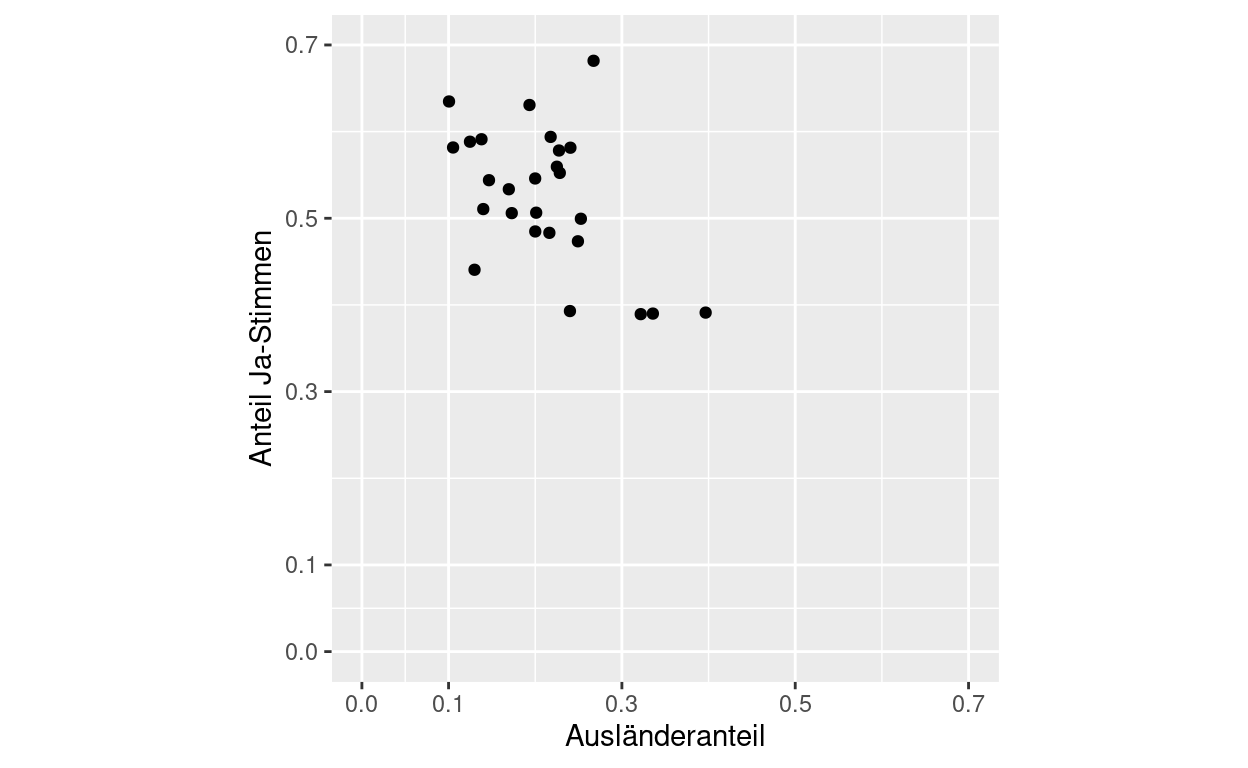
\includegraphics{solution_stat1_files/figure-latex/unnamed-chunk-3-1.pdf}

\begin{Shaded}
\begin{Highlighting}[]
\CommentTok{# führt einen t-Tests durch; }
\CommentTok{# es wird angenommen, dass die Verkaufszahlen zwischen den Bedingungen unabhängig sind}

\NormalTok{t_test <-}\StringTok{ }\KeywordTok{t.test}\NormalTok{(df[df}\OperatorTok{$}\NormalTok{condit }\OperatorTok{==}\StringTok{ "Basis"}\NormalTok{, ]}\OperatorTok{$}\NormalTok{tot_sold, }
\NormalTok{                 df[df}\OperatorTok{$}\NormalTok{condit }\OperatorTok{==}\StringTok{ "Intervention"}\NormalTok{, ]}\OperatorTok{$}\NormalTok{tot_sold)}
\NormalTok{t_test}
\end{Highlighting}
\end{Shaded}

\begin{verbatim}
## 
##  Welch Two Sample t-test
## 
## data:  df[df$condit == "Basis", ]$tot_sold and df[df$condit == "Intervention", ]$tot_sold
## t = 1.5367, df = 3.5781, p-value = 0.2074
## alternative hypothesis: true difference in means is not equal to 0
## 95 percent confidence interval:
##  -8.343572 27.010238
## sample estimates:
## mean of x mean of y 
##  190.6667  181.3333
\end{verbatim}

\hypertarget{methoden-1}{%
\paragraph{Methoden}\label{methoden-1}}

Ziel war es die wöchentlichen Verkaufszahlen zwischen den Interventions-
und Basiswochen zu vergleichen. Die Annahme war, dass die wöchentlichen
Verkaufszahlen unabhängig sind. Daher können die mittleren
Verkaufszahlen pro Woche zwischen den beiden Bedingungen mittels t-Test
geprüft werden. Obwohl die visuelle Inspektion keine schwerwiegenden
Verletzungen der Modelvoraussetzung zeigte, wurde einen Welch t-Test
gerechnet.

\hypertarget{ergebnisse-1}{%
\paragraph{Ergebnisse}\label{ergebnisse-1}}

In den Basiswochen werden mehr Gerichte pro Woche verkauft als in den
Interventionsowochen (siehe Figure 1). Die wöchentlichen Verkaufszahlen
zwischen den Bedigungen (Basis oder Intervention) unterscheiden sich
gemäss Welch t-Test jedoch nicht signifikant (\emph{t}(4) = 1.537 ,
\emph{p} = 0.207).

\begin{figure}
\centering
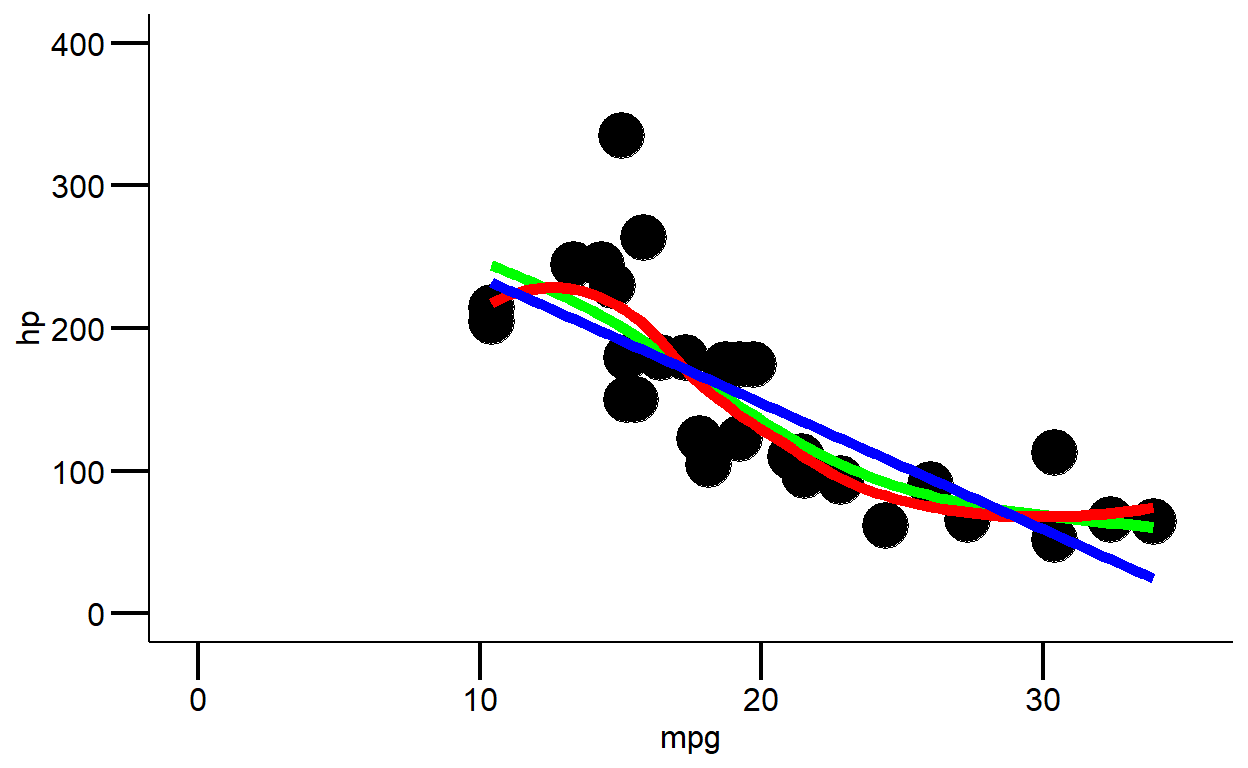
\includegraphics{solution_stat1_files/figure-latex/unnamed-chunk-5-1.pdf}
\caption{Die wöchentlichen Verkaufszahlen für die Interventions- und
Basiswochen unterscheiden sich nicht signifikant.}
\end{figure}


\end{document}
